\documentclass[10pt,a4paper]{article}

\usepackage[utf8]{inputenc}
\usepackage[T1]{fontenc}
\usepackage[spanish,es-tabla]{babel}
\usepackage[margin=1.55cm,top=1.45cm,bottom=1.55cm]{geometry}
\usepackage{amsmath}
\usepackage{array}
\usepackage{booktabs}
\usepackage{tabularx}
\usepackage{graphicx}
\usepackage{xcolor}
\usepackage{xurl}
\usepackage[colorlinks=true,linkcolor=blue!60!black,urlcolor=blue!60!black]{hyperref}

\setlength{\parskip}{3pt}
\setlength{\parindent}{0pt}

\newcommand{\incluircaptura}[2]{%
  \IfFileExists{img/#2}{\includegraphics[width=#1]{img/#2}}{%
    \IfFileExists{docs/img/#2}{\includegraphics[width=#1]{docs/img/#2}}{%
      \fbox{\parbox[c][2.6cm][c]{0.92\linewidth}{\centering\footnotesize Captura pendiente: \texttt{docs/img/\detokenize{#2}}.}}%
    }%
  }%
}

\begin{document}

\begin{center}
    {\large \textbf{UNIVERSIDAD TÉCNICA ESTATAL DE QUEVEDO}} · Facultad de Ciencias de la Computación · Ingeniería en Software\\[0.08cm]
    \rule{\linewidth}{0.45mm}\\[0.14cm]
    {\Large \textbf{AP-U1 · AforoSeguro: Control de Aforo Distribuido}}\\[0.08cm]
    {\small Aplicaciones Distribuidas (ISR-701) · SPA 2026--2027 · Docente: Gleiston C. Guerrero-Ulloa, PhD}\\[0.06cm]
    {\small \textbf{Estudiante:} Luis Jeremy Jaramillo Acosta (\texttt{@JeremyJaramillo72}) · \textbf{Fecha:} 23/11/2026 · \textbf{Códigos:} \texttt{KD55-TB} / \texttt{662D\_M6}}\\[0.05cm]
    {\footnotesize \textbf{Repositorio:} \url{https://github.com/JeremyJaramillo72/AP-U1-Jaramillo-Jeremy}}\\[0.08cm]
    \rule{\linewidth}{0.45mm}
\end{center}

\vspace{-0.12cm}
\noindent\textbf{Resumen del prototipo.} El sistema consta de un coordinador (ID~\texttt{0}) y tres puertas (\texttt{P1 Norte}, \texttt{P2 Sur} y \texttt{P3 Este}, IDs~\texttt{1}, \texttt{2} y \texttt{3}) comunicados en Java mediante sockets TCP. Cada mensaje JSON termina en salto de línea (\texttt{\textbackslash n}) con \texttt{PrintWriter.println} y \texttt{BufferedReader.readLine} para que las solicitudes no se mezclen ni se corten. Todas las peticiones llevan el \texttt{token} de \texttt{config.properties}; el contador \texttt{dentro} se protege con \texttt{synchronized (lockAforo)}; las puertas mandan un latido cada 2\,s (timeout de caída en 6\,s) y cada proceso guarda su bitácora en \texttt{logs/<proceso>.log} con reloj lógico de Lamport.

\section*{1. Escenarios ejecutados y capturas}
\vspace{-0.15cm}

En la Tabla~\ref{tab:escenarios} se resumen los escenarios ejecutados (\texttt{E0} a \texttt{E6}), su captura correspondiente y lo observado en cada prueba.

\begin{table}[htbp]
\centering
\caption{Escenarios ejecutados (E0 a E6) y lo observado en el prototipo.}
\label{tab:escenarios}
\footnotesize
\setlength{\tabcolsep}{4pt}
\begin{tabularx}{\textwidth}{>{\bfseries}l c X}
\toprule
Esc. & Captura & Observación e interpretación \\
\midrule
E0 & Fig.~\ref{fig:e0} & Se comprobó con \texttt{Get-NetAdapter} que \texttt{Ethernet} y \texttt{Wi-Fi} estaban en estado \texttt{Disconnected} al inicio de la práctica y se hizo el primer \emph{commit} con el código \texttt{KD55-TB}. \\
E1 & Fig.~\ref{fig:e1} & Al arrancar P1, P2 y P3, el coordinador las marcó como \texttt{ACTIVA} al recibir sus primeros latidos. Entraron personas por las tres puertas (\texttt{1/10}, \texttt{2/10}, \texttt{3/10}), salió una por P2 (\texttt{2/10}) y el comando \texttt{estado} mostró el mismo total global y las tres puertas activas. \\
E2 & Fig.~\ref{fig:e2} & Al vaciar el aforo, una salida extra devolvió \texttt{RECHAZADA (nadie dentro)}. Luego se registraron 10 entradas seguidas (\texttt{1/10} a \texttt{10/10}); la entrada 11 desde P1 fue \texttt{RECHAZADA (aforo completo)}. Por último, \texttt{token\_mal} fue rechazada por \texttt{token invalido} y quedó en \texttt{logs/coordinador.log} como \texttt{1121;0;TOKEN\_INVALIDO}. \\
E3 & Fig.~\ref{fig:e3} & Al lanzar 30 hilos simultáneos con \texttt{PruebaCarga} y aforo 10, el coordinador normal dejó pasar \textbf{10} y rechazó \textbf{20} (contador final \textbf{10}). En modo \texttt{-inseguro} dejó pasar las \textbf{30}, no rechazó ninguna y el contador quedó en \textbf{29} (ver Tabla~\ref{tab:e3}). \\
E4 & Fig.~\ref{fig:e4} & Al cerrar P3 (\texttt{cerrar}), pasados los 6\,s sin latidos el coordinador mostró \texttt{[ALERTA] Puerta P3 marcada como CAIDA} (\texttt{2717;0;PUERTA\_CAIDA}). Al volver a ejecutar P3, su primer latido la cambió de nuevo a \texttt{ACTIVA} (\texttt{2775;0;PUERTA\_ACTIVA}) y \texttt{estado} en P1 la mostró activa otra vez. \\
E5 & Fig.~\ref{fig:e5} & Con las puertas activas se detuvo el coordinador y se probó \texttt{entrar} en P1. Al fallar el socket TCP, P1 rechazó la operación en local (\texttt{2418;1;RECHAZO\_LOCAL}) para no arriesgar un sobrepaso del aforo. \\
E6 & Fig.~\ref{fig:e6} & \texttt{OrdenTotal} juntó los cuatro archivos de \texttt{logs/} y generó \texttt{logs/orden\_total.log} con \textbf{5910 eventos} ordenados por marca de Lamport y desempatados por \texttt{id\_proceso} (por ejemplo, \texttt{1;0} a \texttt{1;3} y en $L=640$). \\
\bottomrule
\end{tabularx}
\end{table}

\begin{figure}[htbp]
\centering
\begin{minipage}[t]{0.485\textwidth}
    \centering
    \incluircaptura{\linewidth}{E0_sin_red.png}
    \caption{Escenario E0: verificación de adaptadores de red desconectados.}
    \label{fig:e0}
\end{minipage}\hfill
\begin{minipage}[t]{0.485\textwidth}
    \centering
    \incluircaptura{\linewidth}{E1_operacion_normal.png}
    \caption{Escenario E1: operación normal con coordinador y puertas P1, P2 y P3 activas.}
    \label{fig:e1}
\end{minipage}
\end{figure}

\begin{figure}[htbp]
\centering
\incluircaptura{0.82\textwidth}{E2_aforo_y_token.png}
\caption{Escenario E2: aforo completo en la 11.\textsuperscript{a} entrada y rechazo de token inválido.}
\label{fig:e2}
\end{figure}

\begin{figure}[htbp]
\centering
\incluircaptura{0.76\textwidth}{E3_carga_concurrente.png}
\caption{Escenario E3: \texttt{PruebaCarga} en modo normal (\texttt{10} permitidas, \texttt{20} rechazadas, contador \texttt{10}; arriba) y en modo \texttt{-inseguro} (\texttt{30} permitidas, \texttt{0} rechazadas, contador \texttt{29}; abajo).}
\label{fig:e3}
\end{figure}

\begin{figure}[htbp]
\centering
\begin{minipage}[t]{0.485\textwidth}
    \centering
    \incluircaptura{\linewidth}{E4_puerta_caida.png}
    \caption{Escenario E4: P3 marcada como \texttt{CAIDA} tras $>6$\,s y reactivada al reiniciarla.}
    \label{fig:e4}
\end{minipage}\hfill
\begin{minipage}[t]{0.485\textwidth}
    \centering
    \incluircaptura{\linewidth}{E5_coordinador_caido.png}
    \caption{Escenario E5: coordinador detenido y rechazo local en P1.}
    \label{fig:e5}
\end{minipage}
\end{figure}

\begin{figure}[htbp]
\centering
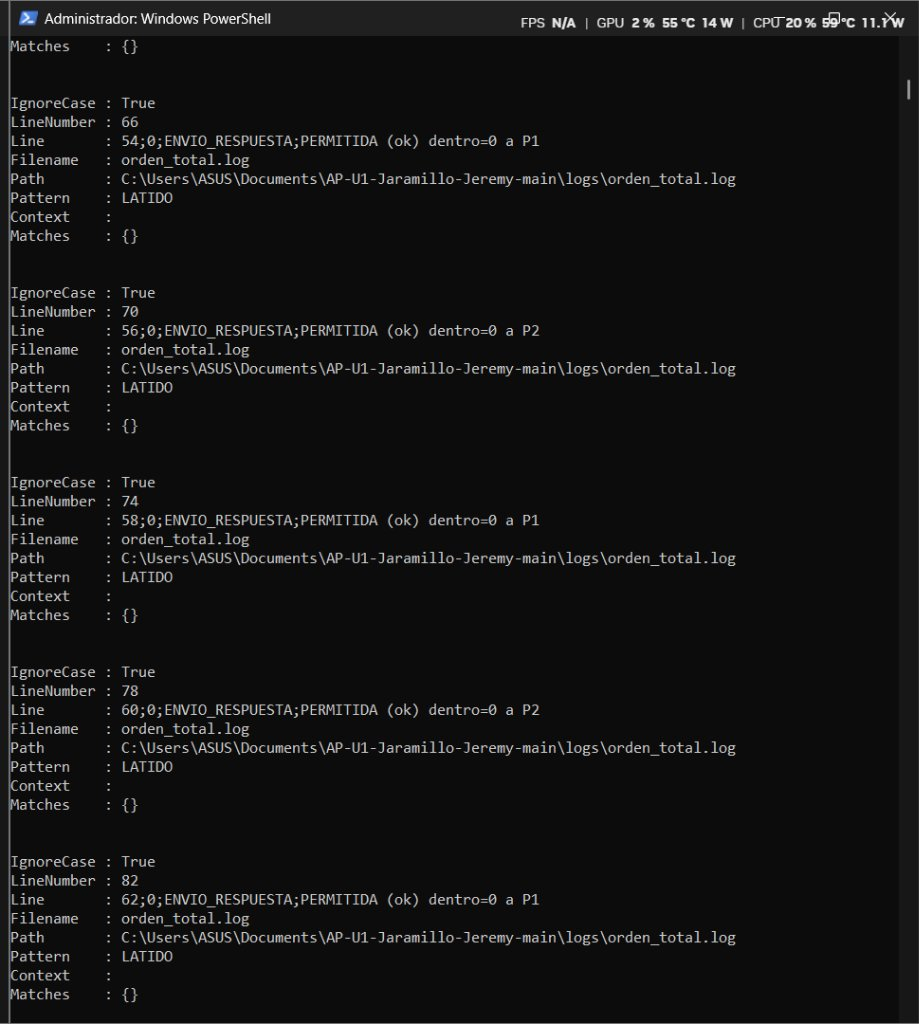
\includegraphics[width=0.58\textwidth,height=5.8cm,keepaspectratio]{img/E6_orden_total.png}
\caption{Escenario E6: salida de \texttt{OrdenTotal} sobre \texttt{logs/orden\_total.log} (5910 eventos).}
\label{fig:e6}
\end{figure}

\section*{2. Cifras de E3 y pares causales de E6}
\vspace{-0.15cm}

La Tabla~\ref{tab:e3} recoge los números obtenidos al ejecutar \texttt{PruebaCarga} (30 solicitudes simultáneas, 10 hilos por puerta, \texttt{aforo=10}) contra el coordinador en modo normal y en modo \texttt{-inseguro}.

\begin{table}[htbp]
\centering
\caption{Resultados de \texttt{PruebaCarga} en el escenario E3 (30 hilos simultáneos, \texttt{aforo=10}).}
\label{tab:e3}
\footnotesize
\begin{tabularx}{\textwidth}{l c c c c X}
\toprule
\textbf{Modo} & \textbf{Permitidas} & \textbf{Rechazadas} & \textbf{Errores} & \textbf{Contador final} & \textbf{Comportamiento observado} \\
\midrule
Normal (\texttt{synchronized}) & 10 & 20 & 0 & 10 & Respeta el límite de 10 personas sin desbordes. \\
Inseguro (\texttt{-inseguro}) & 30 & 0 & 0 & 29 & Se desbordó en 20 entradas y se perdió 1 incremento ($29 \neq 30$). \\
\bottomrule
\end{tabularx}
\end{table}

Con los registros de E1 a E5, \texttt{OrdenTotal} generó \texttt{logs/orden\_total.log} con 5910 líneas. En la Tabla~\ref{tab:causales} se muestran dos pares de eventos reales tomados directamente de ese archivo donde el envío aparece antes que su recepción ($L_{\text{envío}} < L_{\text{recepción}}$).

\begin{table}[htbp]
\centering
\caption{Dos pares causales verificados en \texttt{logs/orden\_total.log} (E6).}
\label{tab:causales}
\scriptsize
\setlength{\tabcolsep}{4pt}
\begin{tabularx}{\textwidth}{>{\bfseries}l c >{\raggedright\arraybackslash}p{6.6cm} X}
\toprule
Par & Línea & Registro en \texttt{logs/orden\_total.log} & Relación causal \\
\midrule
Par 1 & 1226 & \texttt{637;2;ENVIO\_ENTRAR;solicitud al coordinador} & P2 sube su reloj a $L=637$ antes de enviar \texttt{ENTRAR}. \\
      & 1227 & \texttt{638;0;RECIBE\_ENTRAR;puerta=P2} & El coordinador recibe $637$ y fija $\max(\text{local},637)+1=638$; se cumple $637 < 638$. \\
\midrule
Par 2 & 1228 & \texttt{639;0;ENVIO\_RESPUESTA;PERMITIDA (ok) dentro=2 a P2} & El coordinador incrementa su reloj a $L=639$ y envía la respuesta. \\
      & 1230 & \texttt{640;2;RECIBE\_RESPUESTA;PERMITIDA (ok) dentro=2} & P2 recibe $639$ y fija $\max(637,639)+1=640$; se cumple $639 < 640$. \\
\bottomrule
\end{tabularx}
\end{table}

En la marca $L=640$ también se ve el desempate por identificador de proceso: la línea~1229 (\texttt{640;0;RECIBE\_LATIDO}) precede a la línea~1230 (\texttt{640;2;RECIBE\_RESPUESTA}) porque el proceso \texttt{0} va antes que el \texttt{2}.

\section*{3. Preguntas de análisis}
\vspace{-0.15cm}

\textbf{1. ¿Por qué el modo \texttt{-inseguro} permitió más entradas que el aforo en E3? ¿Qué mecanismo lo evita en modo normal y qué costo tiene?}
En \texttt{-inseguro} el coordinador dejó pasar las 30 solicitudes y terminó marcando \texttt{dentro=29} por dos condiciones de carrera. Primero, como no hay bloqueo entre la comprobación \texttt{if (dentro < config.aforo)} y el incremento, y además hay un \texttt{Thread.sleep(50)}, los 30 hilos vieron \texttt{dentro} menor a 10 al mismo tiempo y pasaron todos. Segundo, \texttt{dentro++} tampoco es atómico, así que dos hilos pisaron su incremento y el contador cerró en 29 aunque se aprobaron 30 entradas. En modo normal, el bloque \texttt{synchronized (lockAforo)} aplica exclusión mutua para que solo un hilo a la vez consulte y actualice \texttt{dentro}, dejando entrar exactamente 10 y rechazando 20. El costo de usar \texttt{synchronized} es que los hilos tienen que esperar turno para entrar a la sección crítica (menor concurrencia bajo mucha carga), aunque aquí esa espera es mínima comparada con el tiempo de abrir el socket TCP.

\textbf{2. En E5, ¿qué priorizó el sistema (consistencia o disponibilidad)? Relación con el teorema CAP y consecuencias.}
Al caer el coordinador, \texttt{Puerta.java} atrapó la \texttt{IOException}, guardó \texttt{2418;1;RECHAZO\_LOCAL} en \texttt{logs/puerta1.log} y negó la entrada con el mensaje de error. Con eso prioricé la \textbf{consistencia (C)} del aforo sobre la \textbf{disponibilidad (A)} de las puertas frente a una caída o partición (\textbf{P}). Según el teorema CAP, si el coordinador queda inalcanzable no se pueden mantener ambas propiedades a la vez: si cada puerta dejara pasar gente por su cuenta (AP), entre las tres pasarían el aforo de 10 sin enterarse. Para el público esto implica que la fila se detiene y nadie entra hasta que el coordinador vuelva; para la administración da seguridad de que nunca se superará el aforo permitido, pero obliga a cuidar que el coordinador no se caiga.

\textbf{3. Punto único de fallo del coordinador: mecanismo de la Unidad~I para tolerarlo y nuevo problema.}
Como todo pasa por el proceso 0, si el coordinador se cae (como en E5) todo el sistema se bloquea. Para que siga trabajando usaría \textbf{replicación primario-respaldo} del coordinador junto con \textbf{elección de líder} (por ejemplo, algoritmo \emph{Bully} o de \emph{Anillo}) y latidos entre réplicas para que un respaldo tome el control si el principal deja de responder. El problema nuevo al tener varias copias del contador \texttt{dentro} es mantener la \textbf{consistencia entre réplicas}: si hay entradas al mismo tiempo o la red se divide (\emph{split-brain}), dos coordinadores podrían llevar cuentas distintas y dejar pasar más personas que el aforo, lo que obliga a sincronizar las réplicas antes de confirmar una entrada.

\textbf{4. Falacia de la computación distribuida en los tiempos de 2\,s y 6\,s, y qué pasaría con 7\,s de latencia.}
Al configurar latidos cada 2\,s y marcar caída a los 6\,s se tuvo en cuenta la falacia \textbf{«la latencia es cero»} (y también \textbf{«la red es fiable»}), dando tres intervalos de margen para pequeños retrasos, pero suponiendo que un mensaje normal tarda menos de 6\,s. Si la red tuviera una latencia de 7\,s pasarían dos cosas en mi código: primero, el timeout del socket en \texttt{Protocolo.enviarYRecibir()} (\texttt{setSoTimeout(3000)}) cortaría cada solicitud antes de recibir respuesta, provocando \texttt{RECHAZO\_LOCAL} y \texttt{LATIDO\_FALLIDO}; segundo, el monitor del coordinador (\texttt{timeoutLatidoMs=6000}) marcaría a las puertas vivas como \texttt{CAIDA} (falsos positivos) y cambiaría repetidamente entre \texttt{CAIDA} y \texttt{ACTIVA} si algún latido retrasado llegara después.

\medskip
\noindent\textbf{Limitaciones del prototipo.}
El contador \texttt{dentro} solo vive en RAM, por lo que al reiniciar el coordinador vuelve a cero sin recuperar el estado anterior. Además, cada conexión crea un hilo nuevo (\texttt{new Thread(...)}) sin límite de piscina de hilos, y el \texttt{token} se envía en texto plano por TCP sin cifrado.

\end{document}
